\chapter{Tune for the primordial $k_T$ events}
\label{chap:primordialkTtune}

The primordial $k_T$ is another important parameter in the description of the proton-proton collisions with Monte Carlo simulations. The primordial $k_T$ description in \textsc{pythia8} was introduced in \secRef{sec:Beam Beam Remnants and primordial kT}.
\\
The main unresolved problem for the primordial $k_T$ tune is the unexpected high value required for the description of the observed $Z$ boson $p_T$ spectrum.
\\
In fact, the primordial $k_T$ si derived by the Fermi Motion of partons inside the hadrons. So when the parton undergoes to the hard scattering it can already have an initial no zero transverse momentum.
The value of the primordial $k_T$ can be estimate as reported in \eqRef{eq:PrimordialKT}, but experimental data for the $Z$ boson $p_T$ spectrum show that this estimation is not sufficient the required value observed in order to reproduce the experimental data are in the order of $2\ \mathrm{GeV}$.
\\
%The introduction of the primordial $k_T$ is really important in the description of the $Z$ boson $p_T$ spectrum. At the LO calculation there is nothing that can recoil against the $Z$ boson so it can only be produced with zero $p_T$. With the introduction of the primordial $k_T$ one have that the already at the LO the $Z$ can have a non zero primordial $k_T$.
%
The primordial $k_T$ was tune in the Monash tune \cite{Monash} and the following tunes, as CP5, inherited the values of the parameters from there.
\\
So the introduction of a new tune for the primordial $k_T$ is needed. In fact the CP5 tune it is known that does not describe well the $Z$ spectrum in the low-$p_T$ region \cite{CPtunes}. This is shown in \figRef{fig:CP5_notdescribeZjet} for the production cross-section in $Z$ plus jets events and in the figure \figRef{fig:CP5_notdescribeZ} for $Z$ boson production in DY observations. As we can se the CP5 tune is very far from experimental data values in the low regions. 
\\
The distribution for $Z+$jets events as a function of the variable $p_T^{bal}=\big|p_T^Z-\sum_{\text{jets}}p_T^{j}\big|$ is not well described in the first bin. While the one as a function of the $p_T^Z$ miss the description in the region $p_T^Z \lesssim 40\ \mathrm{GeV}$. This two observable as described in \cite{CPtunes} are very sensitive to the parton shower process and so to the UE.
\\
For the tune we focus on the distributions in \figRef{fig:CP5_notdescribeZ} were the effects of MPI is expected to be less important\footnote{below it is preliminarily investigate the effect of the MPI on these distributions. This aspect is never been investigated into detail and require further studies maybe also the inclusion of data from \textsc{lhc} \textsc{run3} can improve the description of these observables.}, also here we can see that CP5 tune don't describe very well the low regions for this two observables.  


\begin{figure}[!htb]
	\centering
	\noindent
	\begin{subfigure}{0.5\textwidth}
		\centering
		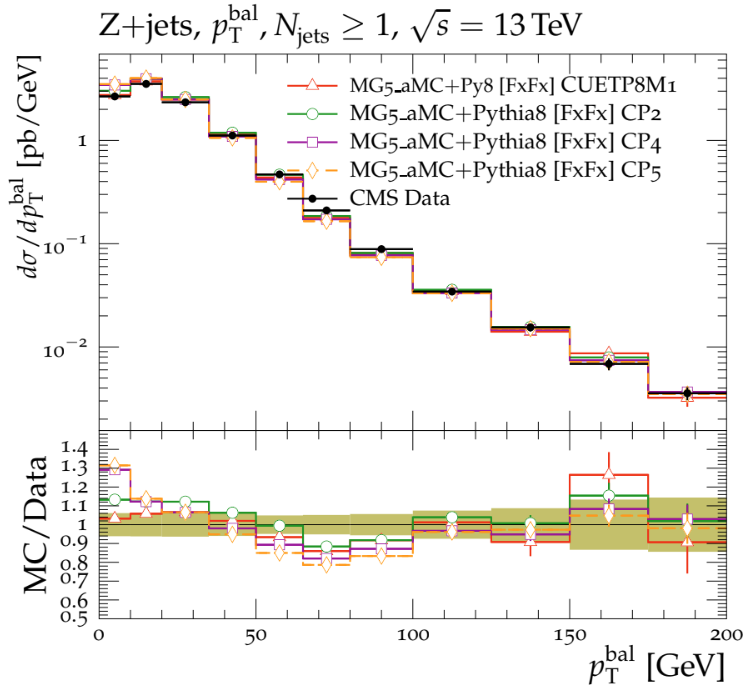
\includegraphics[width=0.985\textwidth]{{img/CPpaper_zjet1.png}}
	\end{subfigure}%
	\begin{subfigure}{0.5\textwidth}
		\centering
		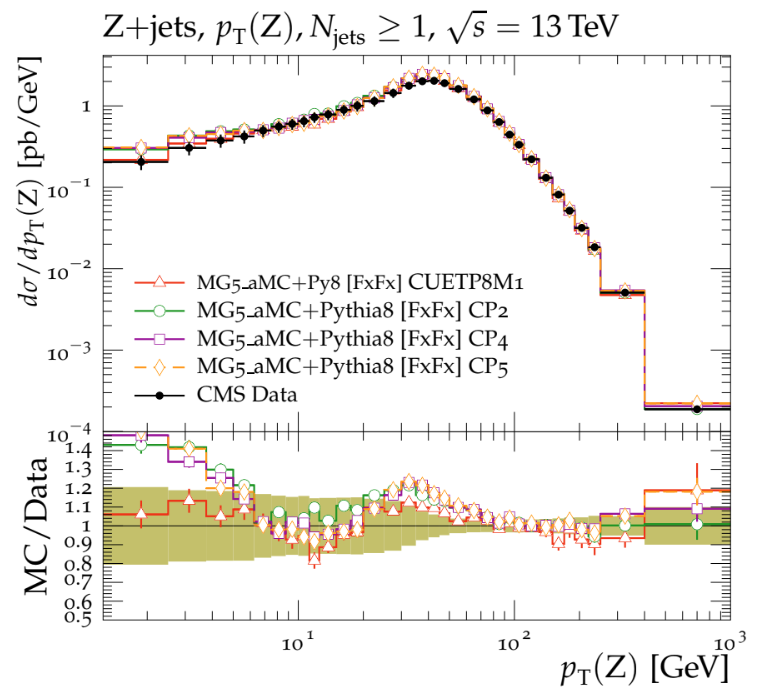
\includegraphics[width=\textwidth]{{img/CPpaper_zjet2.png}}
	\end{subfigure}%
	\caption{Figure from CP tunes presentation paper \cite{CPtunes}. These two images show the $Z$ boson production cross-section in $Z$ plus jets (with at least one jet) at $\sqrt{s}=13\ \mathrm{TeV}$ as a function of the imbalance of the transverse momentum between the jet and the $Z$ boson (left) and of the $Z$ boson transverse momentum (right) \cite{CMS:2018mdf}. The first bin in the left distribution and the regione $p_T^Z \lesssim 40\ \mathrm{GeV}$ in the right one are not well described by CP5 tune (yellow line).}
	\label{fig:CP5_notdescribeZjet}
\end{figure}

\begin{figure}[!htb]
	\centering
	\noindent
	\begin{subfigure}{0.5\textwidth}
		\centering
		\includegraphics[width=\textwidth]{{img/rivet-plots-PrimordialkT_only_CP5default/CMS_2019_I1753680/d27-x01-y03.pdf}}
	\end{subfigure}%
	\begin{subfigure}{0.5\textwidth}
		\centering
		\includegraphics[width=\textwidth]{{img/rivet-plots-PrimordialkT_only_CP5default/CMS_2019_I1753680/d28-x01-y03.pdf}}
	\end{subfigure}
	\caption{The CP5 tune is not good in the description of the low region of the $Z$ boson production cross-section of the $Z$ boson transverse momentum (left) or of the $\phi_\eta^*$ angle. This distribution are from the CMS analysis \cite{ZpT_distributions} at the center-of-mass energy of $13\ \mathrm{TeV}$.}
	\label{fig:CP5_notdescribeZ}
\end{figure}

\section{Primordial $k_T$ and ISR effect on $p_T^Z$}

The parameters on which we focus in order to tune data and explain the $Z$ boson $p_T$ spectrum are:
\begin{itemize}
\item \texttt{BeamRemnants:primordialKThard} that set the width of the Gaussian distribution for the primordial $k_T$ sample;
\item \texttt{SpaceShower:pT0Ref} that set the threshold for the initial state radiation to take place.
\end{itemize}
Let discuss how this parameter impact on the $Z$ boson production transverse momentum spectrum. If we consider only the LO diagram for the $Z$ production (\figRef{fig:feynamn_primkT_Zboson}a) we can have only a production with a zero transverse momentum. So the $Z$ spectrum we expect at LO is a $\delta$-distribution function centered on zero.  

\begin{figure}[!htb]
	\centering
	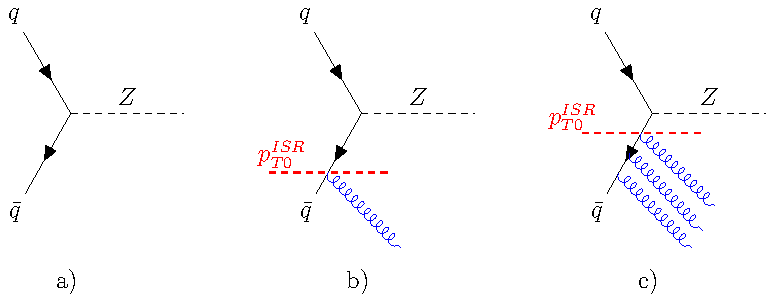
\includegraphics[width=0.8\textwidth]{{img/feynman_ZpT_2_blue.pdf}}
	\caption{$Z$ boson production diagrams: a) shows the LO diagram; b) is the LO diagram whit a high threshold for the ISR so we have a small amount; c) is the same but with a lower threshold for the ISR and a larger amount, in b) and c) cases the $Z$ boson can be produced with a non-zero transverse momentum, balanced by the ISR.}
	\label{fig:feynamn_primkT_Zboson}
\end{figure}

\noindent With the addition of the primordial $k_T$ we get a Gaussian distribution which width is set by \texttt{BeamRemnants:primordialKThard}.
If we move to higher order diagrams the $Z$ boson can be produced with a non zero $p_T$ that is balanced by the various jets, then the primordial $k_T$ is added to the already non-zero $Z$ boson transverse momentum. 
\\
A large contribution come also from the amount of ISR that is emitted from the incoming partons, in fact each split can give to the incoming parton a non-zero initial value of $p_T$ and so the $Z$ boson is created with a non-zero $p_T$ before the introduction of the primordial $k_T$. 
\\
An higher amount of ISR, so a lower value for the threshold, can lead to a larger $p_T$ taken from the parton that then can generate the $Z$ boson with an higher $p_T$ and vice versa.

\section{Primordial $k_T$ tune}

The primordial $k_T$ was not investigated by CP5 so it is important to include that in the analysis in order to describe better the low $p_T$ region. 

The parameters variation ranges we use are the one reported in the \tableRef{table:primordialkT_variations} while others parameters are set to CP5 values.



\begin{table}[!htb]
\centering
\begin{tabular}{l | c }
Parameter Name & Value \\ 
\hline \hline
\\[-0.85em]
	\texttt{BeamRemnants:primordialKThard} & $[0.5 - 5.0]$\\[2pt]
	\texttt{SpaceShower:pT0Ref} & $[0.5 - 5.0]$\\
\end{tabular}
\caption{Variation ranges for the sampling used in the primordial $k_T$ tune.}
\label{table:primordialkT_variations}
\end{table} 

The number of samples is lower than the one used for the Underlying Event in fact the training set we use for the PerBin Model contains more or less $160$ MC runs and a little more for the Inverse Model, $\sim 200$, this is realated to the lower number of parameters to tune. So, the operation for the tune was computationally faster.
\\
\figRef{fig:CP5_notdescribeZ} shows the distributions used to performed the tune. The distributions  are from the \cite{ZpT_distributions} analysis at $\sqrt{s}=13\ \mathrm{TeV}$:
\begin{itemize}
	\item The $Z$ boson production cross-section in DY observation as a function of $p_T^Z$;
	\item The $Z$ boson production cross-section in DY observation as a function of $\phi_\eta^*$.
\end{itemize}

\noindent Note that: the region of interest is the low $p_T$ region. The simulation of the whole spectrum requires the adoption of a higher order merging scheme between the higher order matrix element calculations and parton shower, as FxFx, that is computationally expensive. So the strategy followed was the tuning of the low region, the one of interest, taking only the first five bins from each distribution.  


\medskip

\noindent The PerBin Model minimization results are displayed in \figRef{fig:result_PerBin_PrimordialkT_1}. The blue line indicates the value of the $\chi^2/DoF$ as a function of the parameter value. The best estimation is marked by a solid red line while the dashed red lines indicate the errors, these results are reported in \tableRef{table:Primordial_kT_results}. Both the parameters are in a well defined minimum so the minimization phase seems work properly. 

\begin{figure}[!htb]
	\centering
	\noindent 
	\begin{subfigure}{0.48\textwidth}
	\centering
		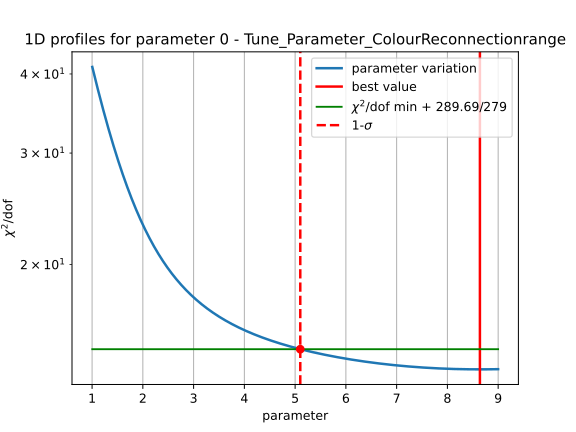
\includegraphics[width=\textwidth]{{img/chi2_0.png}}
	\end{subfigure}%
	\begin{subfigure}{0.48\textwidth}
	\centering
		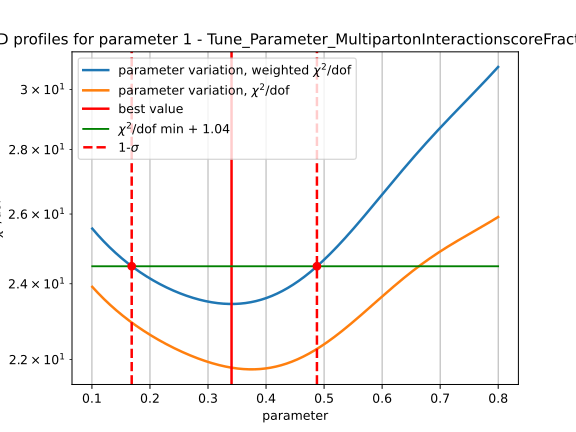
\includegraphics[width=\textwidth]{{img/chi2_1.png}}
	\end{subfigure}
	\caption{The output of the minimizer for the PerBin model in the primordial $k_T$ tune. The left panel shows the result of the minimization for the \texttt{SpaceShower:pT0Ref} parameter while the right one \texttt{BeamRemnants:primordialKThard}. The blue line is the $\chi^2/\mathrm{DoF}$ the best value is indicated by the solid red line while the errors are the ones indicated by the dashed red lines.}
	\label{fig:result_PerBin_PrimordialkT_1}
\end{figure}

\medskip

The Inverse model distribution of prediction for the best model is reported in \figRef{fig:PrimordialkT_InverseModel_results} the best estimation for the parameter is indicated by the solid black line while the dashed black lines are the errors computed using the standard deviation. The hyperparameters space scanned to search for these best model is the same used above and reported in \tableRef{table:hyperpar_MinBias_2par}. AT the end of the scanning the best hyperparameters we found are the one reported in the \tableRef{table:hyperpar_PrimkT}.


\begin{figure}[!htb]
	\centering
	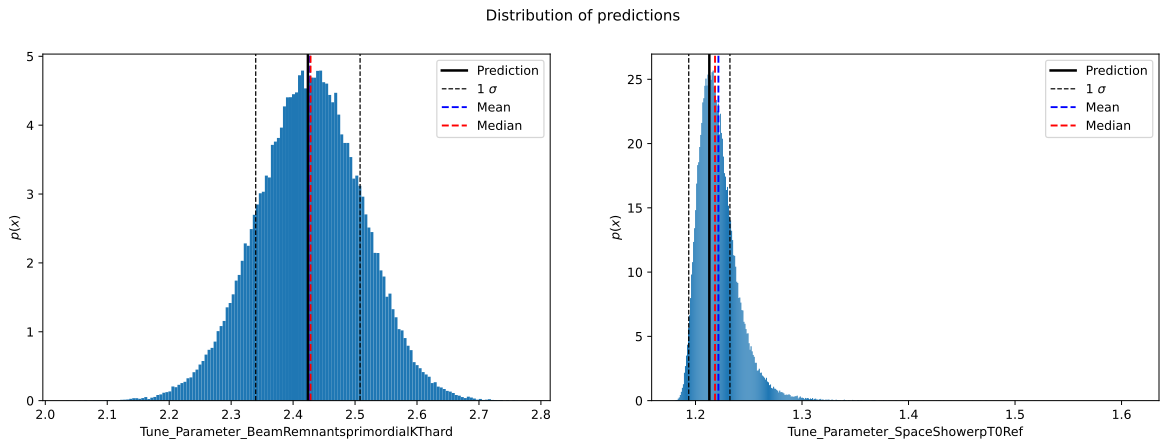
\includegraphics[width=0.95\textwidth]{{img/prediction_spread.png}}
	\caption{The prediction spread for the Inverse model in the primordial $k_T$ tune. The left histograms refers to the \texttt{BeamRemnants:primordialKThard} parameter while the right one to the \texttt{SpaceShower:pT0Ref}. The predictions are indicated by the solid black vertical lines and the errors by the dashed black lines. }
	\label{fig:PrimordialkT_InverseModel_results}
\end{figure}

\begin{table}[!htb]
	\centering
	\begin{tabular}{ l | c }
	Hyperparameter & Value\\[2pt]\hline\hline
	Number of hidden layer & 2 \\[2pt]
	Units layers & [15,\,17] \\[2pt]
	Activation function & sigmoid \\[2pt]
	Optimizer & rmsprop\\[2pt]
	Epochs & 2000\\[2pt]
	Batch size & 64\\[2pt]
	\end{tabular}
	\caption{Best hyperparameters model found for the primordial $k_T$ tune with Inverse model.}
	\label{table:hyperpar_PrimkT}
\end{table}


\noindent The PerBin Model gives to us very stable results the value and the errors we got from the tune are reported in \tableRef{table:Primordial_kT_results}.  
This are also compared to the ones obtained from the Inverse model. The value obtained from the two \textsc{mcnntunes} model are compatible each other. The default values for CP5 are also reported and they are the one inherited by Monash tune \cite{Monash}. As we can see the value we get are quite different to the one in CP5.  

\begin{table}
	\centering
\begin{tabular}{l | c | c | c}
Parameter Name & PerBin & Inverse & Default CP5\\ 
\hline \hline
\\[-0.85em]
	\texttt{BeamRemnants:primordialKThard} & $ 2.5^{+0.2}_{-0.2} $ & $ 2.42\pm0.08 $ & $1.8$\\
	\texttt{SpaceShower:pT0Ref} & $ 1.6^{+0.5}_{-0.5} $ & $ 1.21\pm0.02  $ & $2.0$
\end{tabular}
\caption{Results obtained from the PerBin and the Inverse model in the tuning of the low region of $Z$ boson production spectra. they are compared to the default for CP5 (inherited from Monash tune.)}
\label{table:Primordial_kT_results}
\end{table}	

\medskip

The overall results are displayed in \figRef{fig:result_primKT_FXFX}. Our tunes describe better the low regions of the two spectrum. These low regions are the one we actually tune the higher $p_T$ region is only simulated using the value obtained from the tune of the first 5 bins in each distribution of  \figRef{fig:result_primKT_FXFX}. To simulate all the spectrum we have to use FxFx mergin scheme in order to avoid the double counting and get a correct result from the simulation.

 

 
%\begin{figure}[!htb]
%	\centering
%	\noindent
%	\begin{subfigure}{0.48\textwidth}
%	\centering
%	\includegraphics[width=\textwidth]{{img/rivet-plots-PrimordialkT_PerBin_vs_Inverse_vs_CP5_FxFx_weights/CMS_2019_I1753680/d27-x01-y03.pdf}}	
%	\end{subfigure}%
%	\begin{subfigure}{0.48\textwidth}
%	\centering
%	\includegraphics[width=\textwidth]{{img/rivet-plots-PrimordialkT_PerBin_vs_Inverse_vs_CP5_FxFx_weights/CMS_2019_I1753680/d28-x01-y03.pdf}}	
%	\end{subfigure}
%	\label{fig:result_primKT_FXFX}
%\end{figure}

\begin{figure}[!htb]
	\centering
	\noindent
	\begin{subfigure}{0.48\textwidth}
	\centering
	\includegraphics[width=\textwidth]{{img/rivet-plots-PrimordialkT_PerBin_vs_Inverse_vs_CP5_FxFx_noWeights/CMS_2019_I1753680/d27-x01-y03.pdf}}	
	\end{subfigure}%
	\begin{subfigure}{0.48\textwidth}
	\centering
	\includegraphics[width=\textwidth]{{img/rivet-plots-PrimordialkT_PerBin_vs_Inverse_vs_CP5_FxFx_noWeights/CMS_2019_I1753680/d28-x01-y03.pdf}}	
	\end{subfigure}
	\caption{The results we get from the tune of the primordial $k_T$. The left figure shows the $Z$ boson production cross-section as a function of the $p_T^Z$.  
The red line refers to the PerBin model tune, the blue line to the Inverse Model and the green line is the CP5 default tune. The black points are the experimental data. The colored vertical lines the statistical uncertainties.
	It is clear that our two tunes better describe the low region respect to the original CP5. }
	\label{fig:result_primKT_FXFX}
\end{figure}

\section{Primordial $k_T$ tune vs MPI}

As discussed above primordial $k_T$ is not the only source of non zero transverse momentum in a LO $Z$ boson production.
This is the reason why we are tuning also the parameter that control the amount of Initial State Radiation. As described above, the ISR can leads to a non zero initial transverse momentum a larger amount of ISR (low \texttt{SpaceShower:pT0Ref}) is related to more splitting occurring in the evolution of the incoming partons before that these partons undergo to the hard scattering in which the $Z$ boson is produced. But this is not the only one process that can leads to a non-zero initial transverse momentum, there are also the MPI that can contribute to this initial transverse momentum. It is not an easy task to understand the effect of MPI on the $p_T$ of the produced $Z$ boson. 

\figRef{fig:result_primKT_MPI1} shows the effect of the MPI on the distributions we use for the tune. The blue line is obtained setting \texttt{PartonLevel:MPI=off} in \textsc{Phytia8} configuration.

\begin{figure}[!htb]
	\centering
	\noindent
	\begin{subfigure}{0.48\textwidth}
	\centering
	\includegraphics[width=\textwidth]{{img/rivet-plots-PrimordialkT_with_without_MPI_yellowBand/CMS_2019_I1753680/d27-x01-y03.pdf}}	
	\end{subfigure}%
	\begin{subfigure}{0.48\textwidth}
	\centering
	\includegraphics[width=\textwidth]{{img/rivet-plots-PrimordialkT_with_without_MPI_yellowBand/CMS_2019_I1753680/d28-x01-y03.pdf}}	
	\end{subfigure}
	\caption{The image shows that MPI have an effect on the two distribution. The blue line is the result without the MPI  (\texttt{PartonLevel:MPI=off}) and the red line with MPI.}
	\label{fig:result_primKT_MPI1}
\end{figure}

The main parameters that controls the number of parton interactions in a single hadron-hadron collision is the \texttt{MultipartonInteractions:}\-\texttt{pT0Ref} parameter. It is clear that the first $2$ or $3$ bins of the left distribution of \figRef{fig:result_primKT_MPI1_pt0} are sensitive to the variation of this parameter. A future thing to do is to investigate the effects of these MPI in more detail and perform a more general tune including them in this description.


\begin{figure}[!htb]
	\centering
	\noindent
	\begin{subfigure}{0.48\textwidth}
	\centering
	\includegraphics[width=\textwidth]{{img/rivet-plots-primordialkT_vs_MPI_finale/CMS_2019_I1753680/d27-x01-y03.pdf}}	
	\end{subfigure}%
	\begin{subfigure}{0.48\textwidth}
	\centering
	\includegraphics[width=\textwidth]{{img/rivet-plots-primordialkT_vs_MPI_finale/CMS_2019_I1753680/d28-x01-y03.pdf}}	
	\end{subfigure}
	\caption{The image shows that MPI have an effect on the two distribution. The blue line is the result without the MPI and the red line with MPI.}
	\label{fig:result_primKT_MPI1_pt0}
\end{figure}


